\chapter{Análisis}
\title{Análisis}
\label{cap:Analisis}

\paragraph{
En este capítulo se analizarán los requisitos del proyecto para, más tarde, poder
realizar el diseño.
}

\title{Actores}
\section{Actores}
\paragraph{
Ya en la sección \ref{sec:actoresRequisitos} se hizo alusión a la existencia de
dos tipos de actores. Ahora se profundizará un poco más en su análisis.
}

\begin{itemize}
  \item \textbf{Ac-1.} Director
  \begin{itemize}
   \item Descripción: es quien decide el tempo que debe seguir la banda y comunicar el pulso
   a los músicos
   \item Características: solo hay uno
   \item Relaciones: conocerá a todos los músicos
   \item Atributos: ninguno
   \item Comentarios: tiene la responsabilidad del correcto funcionamiento del sistema
  \end{itemize}

  \item \textbf{Ac-1.} Músico
  \begin{itemize}
     \item Descripción: recibe el pulso del director
     \item Características: hay muchos
     \item Relaciones: conocerá al director. No necesita conocer al resto de músicos
     \item Atributos: ninguno
     \item Comentarios: recibirá el pulso enviado por el director con algún tipo de actuador
  \end{itemize}
\end{itemize}

\title{Casos de uso}
\section{Casos de uso}

\paragraph{
Los casos de uso nos permiten conocer cómo los actores del sistema lo utilizan, en otras
palabras, qué funciones tienen disponibles en el sistema.
}

\title{Descripción de los casos de uso}
\subsection{Descripción de los casos de uso}

\begin{table}[!htbp]
\centering
\label{CU1}
\begin{tabular}{|
>{\columncolor[HTML]{CBCEFB}}l |l|l|}
\hline
{\bf Caso de uso}   & Encender sistema                                    & {\it CU.1}                             \\ \hline
{\bf Actores}       & \multicolumn{2}{l|}{Director,Músico}                                                                \\ \hline
{\bf Tipo}          & \multicolumn{2}{l|}{Primario, esencial}                                                      \\ \hline
{\bf Precondición}  & \multicolumn{2}{l|}{}                                                                        \\ \hline
{\bf Postcondición} & \multicolumn{2}{l|}{El sistema quedará listo para usarse}                                    \\ \hline
{\bf Propósito}     & \multicolumn{2}{l|}{Iniciar el sistema}                                                      \\ \hline
{\bf Resumen}       & \multicolumn{2}{l|}{\begin{tabular}[c]{@{}l@{}}Cada actor iniciará su parte \\
del sistema\end{tabular}} \\ \hline
{\bf Autor}         & Israel Blancas Álvarez                              & Versión 1.0                            \\ \hline
\end{tabular}
\caption{Caso de uso 1}
\end{table}

\begin{table}[!htbp]
\centering
\label{CU2}
\begin{tabular}{|
>{\columncolor[HTML]{CBCEFB}}l |l|l|}
\hline
{\bf Caso de uso}   & Insertar tempo                                                          & {\it CU.2}                                                 \\ \hline
{\bf Actores}       & \multicolumn{2}{l|}{Director}                                                                                                        \\ \hline
{\bf Tipo}          & \multicolumn{2}{l|}{Primario, esencial}                                                                                              \\ \hline
{\bf Precondición}  & \multicolumn{2}{l|}{El sistema debe haberse encendido}                                                                               \\ \hline
{\bf Postcondición} & \multicolumn{2}{l|}{El sistema guardará el tempo}                                                                                    \\ \hline
{\bf Propósito}     & \multicolumn{2}{l|}{Guardar tempo}                                                                                                   \\ \hline
{\bf Resumen}       & \multicolumn{2}{l|}{\begin{tabular}[c]{@{}l@{}} El sistema guardará \\
el tempo indicado por el director\end{tabular}} \\ \hline
{\bf Autor}         & Israel Blancas Álvarez                                                  & Versión 1.0                                                \\ \hline
\end{tabular}
\caption{Caso de uso 2}
\end{table}

\begin{table}[!htbp]
\centering
\label{CU3}
\begin{tabular}{|
>{\columncolor[HTML]{CBCEFB}}l |l|l|}
\hline
{\bf Caso de uso}   & Enviar pulso                           & {\it CU.3}                \\ \hline
{\bf Actores}       & \multicolumn{2}{l|}{Director}                              \\ \hline
{\bf Tipo}          & \multicolumn{2}{l|}{Primario, esencial}                            \\ \hline
{\bf Precondición}  & \multicolumn{2}{l|}{Debe haberse insertado un tempo en el sistema} \\ \hline
{\bf Postcondición} & \multicolumn{2}{l|}{El pulso será comunicado a los músicos}        \\ \hline
{\bf Propósito}     & \multicolumn{2}{l|}{Enviar pulso desde el director a los músicos}  \\ \hline
{\bf Resumen}       & \multicolumn{2}{l|}{\begin{tabular}[c]{@{}l@{}} El pulso es enviado desde el
director a los músicos\end{tabular}}                                              \\ \hline
{\bf Autor}         & Israel Blancas Álvarez                 & Versión 1.0               \\ \hline
\end{tabular}
\caption{Caso de uso 3}
\end{table}

\begin{table}[!htbp]
\label{CU4}
\begin{tabular}{|
>{\columncolor[HTML]{CBCEFB}}l |l|l|}
\hline
{\bf Caso de uso}   & Atender al tempo                                 & {\it CU.4}                         \\ \hline
{\bf Actores}       & \multicolumn{2}{l|}{Músico}                                                           \\ \hline
{\bf Tipo}          & \multicolumn{2}{l|}{Primario, esencial}                                               \\ \hline
{\bf Precondición}  & \multicolumn{2}{l|}{El Director debe estar transmitiendo el pulso}                    \\ \hline
{\bf Postcondición} & \multicolumn{2}{l|}{El Músico conocerá el pulso y quedará sincronizado}               \\ \hline
{\bf Propósito}     & \multicolumn{2}{l|}{Sincronizar al sistema}                                           \\ \hline
{\bf Resumen}       & \multicolumn{2}{l|}{Músico recibirá el pulso}  \\ \hline
{\bf Autor}         & Israel Blancas Álvarez                           & Versión 1.0                        \\ \hline
\end{tabular}
\caption{Caso de uso 4}
\end{table}

\begin{table}[!htbp]
  \centering
\label{CU5}
\begin{tabular}{|
>{\columncolor[HTML]{CBCEFB}}l |l|l|}
\hline
{\bf Caso de uso}   & Percibir el tempo                              & {\it CU.5}                         \\ \hline
{\bf Actores}       & \multicolumn{2}{l|}{Músico}                                                           \\ \hline
{\bf Tipo}          & \multicolumn{2}{l|}{Primario, esencial}                                               \\ \hline
{\bf Precondición}  & \multicolumn{2}{l|}{El músico debe estar recibiendo el pulso del director} \\ \hline
{\bf Postcondición} & \multicolumn{2}{l|}{El músico sentirá el pulso}               \\ \hline
{\bf Propósito}     & \multicolumn{2}{l|}{Seguir el pulso}                                           \\ \hline
{\bf Resumen}       & \multicolumn{2}{l|}{\begin{tabular}[c]{@{}l@{}} Músico recibirá el pulso \\
que le marque el sistema (de forma constante)\end{tabular}}  \\ \hline
{\bf Autor}         & Israel Blancas Álvarez                           & Versión 1.0                        \\ \hline
\end{tabular}
\caption{Caso de uso 5}
\end{table}

\begin{table}[!htbp]
  \centering
\label{CU6}
\begin{tabular}{|
>{\columncolor[HTML]{CBCEFB}}l |l|l|}
\hline
{\bf Caso de uso}   & Detener la comunicación                                & {\it CU.6}                         \\ \hline
{\bf Actores}       & \multicolumn{2}{l|}{Director}                                                           \\ \hline
{\bf Tipo}          & \multicolumn{2}{l|}{Primario, esencial}                                               \\ \hline
{\bf Precondición}  & \multicolumn{2}{l|}{El sistema debe estar encendido}                    \\ \hline
{\bf Postcondición} & \multicolumn{2}{l|}{El director dejará de enviar el pulso}               \\ \hline
{\bf Propósito}     & \multicolumn{2}{l|}{Detener la comunicación}                                           \\ \hline
{\bf Resumen}       & \multicolumn{2}{l|}{\begin{tabular}[c]{@{}l@{}} Músico podrá dejar de recibir el pulso una vez que \\
todos los músicos estén sincronizados. El director \\ detendrá la comunicación apagando el dispositivo\end{tabular}}  \\ \hline
{\bf Autor}         & Israel Blancas Álvarez                           & Versión 1.0                        \\ \hline
\end{tabular}
\caption{Caso de uso 6}
\end{table}


\begin{table}[!htbp]
  \centering
\label{CU7}
\begin{tabular}{|
>{\columncolor[HTML]{CBCEFB}}l |l|l|}
\hline
{\bf Caso de uso}   & Apagar el dispositivo                              & {\it CU.7}                         \\ \hline
{\bf Actores}       & \multicolumn{2}{l|}{Músico}                                                           \\ \hline
{\bf Tipo}          & \multicolumn{2}{l|}{Primario, esencial}                                               \\ \hline
{\bf Precondición}  & \multicolumn{2}{l|}{El director debe haber finalizado el envío del pulso}                    \\ \hline
{\bf Postcondición} & \multicolumn{2}{l|}{El sistema quedará apagado}               \\ \hline
{\bf Propósito}     & \multicolumn{2}{l|}{Apagar el sistema}                                           \\ \hline
{\bf Resumen}       & \multicolumn{2}{l|}{\begin{tabular}[c]{@{}l@{}} Una vez que la \\
comunicación haya finalizado por parte del director,\\ los músicos podrán apagar el sistema (indicándolo)\end{tabular}}  \\ \hline
{\bf Autor}         & Israel Blancas Álvarez                           & Versión 1.0                        \\ \hline
\end{tabular}
\caption{Caso de uso 7}
\end{table}

\clearpage

\subsection{Módulos}
\title{Módulos}
\paragraph{Las funciones del sistema se pueden clasificar, según
las tareas que se realicen, en módulos. Esta separación se representa gráficamente
con un diagrama de paquetes como el de la figura \ref{fig:diagramapaquetes}}

\begin{figure}[!htb]
\centering
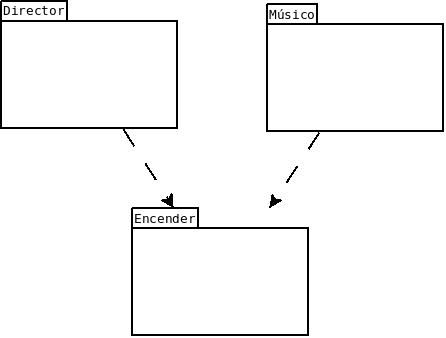
\includegraphics[width=1\textwidth]{./imagenes/diagramapaquetes}
\caption{Diagrama de paquetes} \label{fig:diagramapaquetes}
\end{figure}

\paragraph{Los casos de uso de podrán clasificar dentro de estos paquetes}

\subsection{Diagrama de casos de uso}
\title{Diagrama de casos de uso}
\paragraph{
Gracias a este diagrama, podemos tener una representación gráfica que nos
indica quién realiza cada caso de uso (y, según la clasificación anterior,
comprender en qué modulo se sitúa dicha acción).
}
\begin{figure}[!htb]
\centering
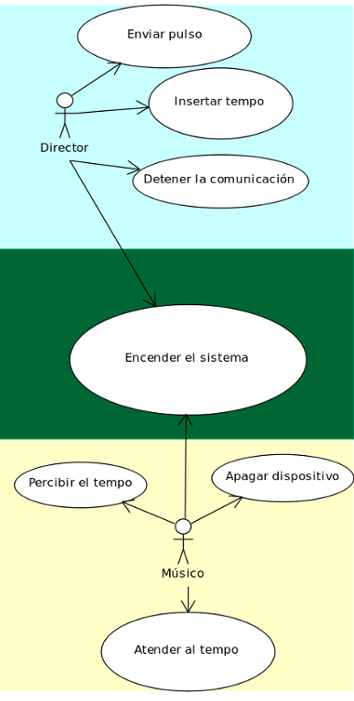
\includegraphics[]{./imagenes/diagramacasosdeuso}
\caption{Diagrama de casos de uso} \label{fig:diagramacasosdeuso}
\end{figure}

\paragraph{
Los casos de uso dentro del cuadro verde corresponden a los del módulo ``Encender".
Aquellos que se encuentran dentro del cuadro de color crema, al módulo ``Músico" y, finalmente,
los de color turquesa, al módulo ``Director".
}
